\section{Progettazione}
In relazione ai requisiti individuati nella sezione precedente, sono state progettate le interfacce che le pagine dovranno avere e la loro architettura ad alto livello.


\subsection{Home}
[descrizione home..]
\begin{figure}[H]
	\centering
	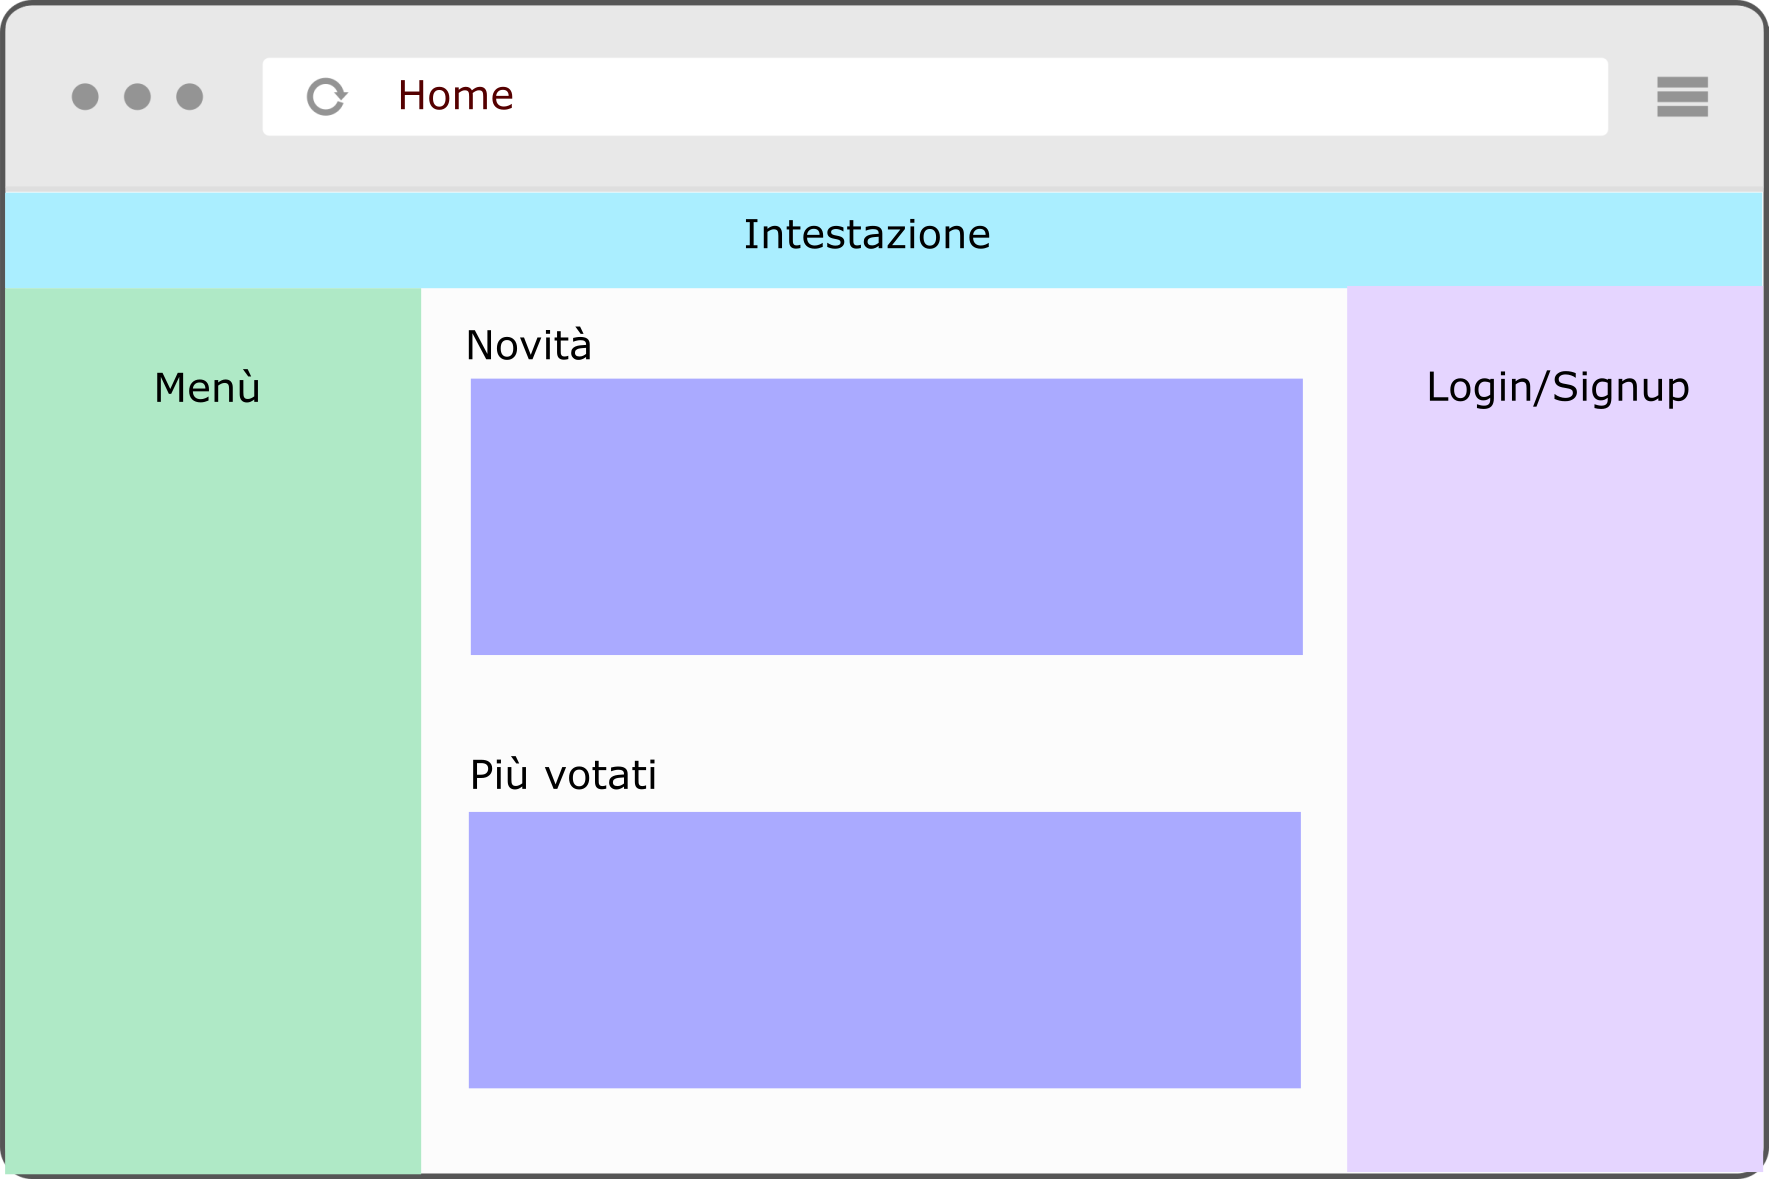
\includegraphics[width= 14cm]{immagini/home.png}
	\caption{Home page}
\end{figure}

\subsection{Catalogo}
[descrizione catalogo..]
\begin{figure}[H]
	\centering
	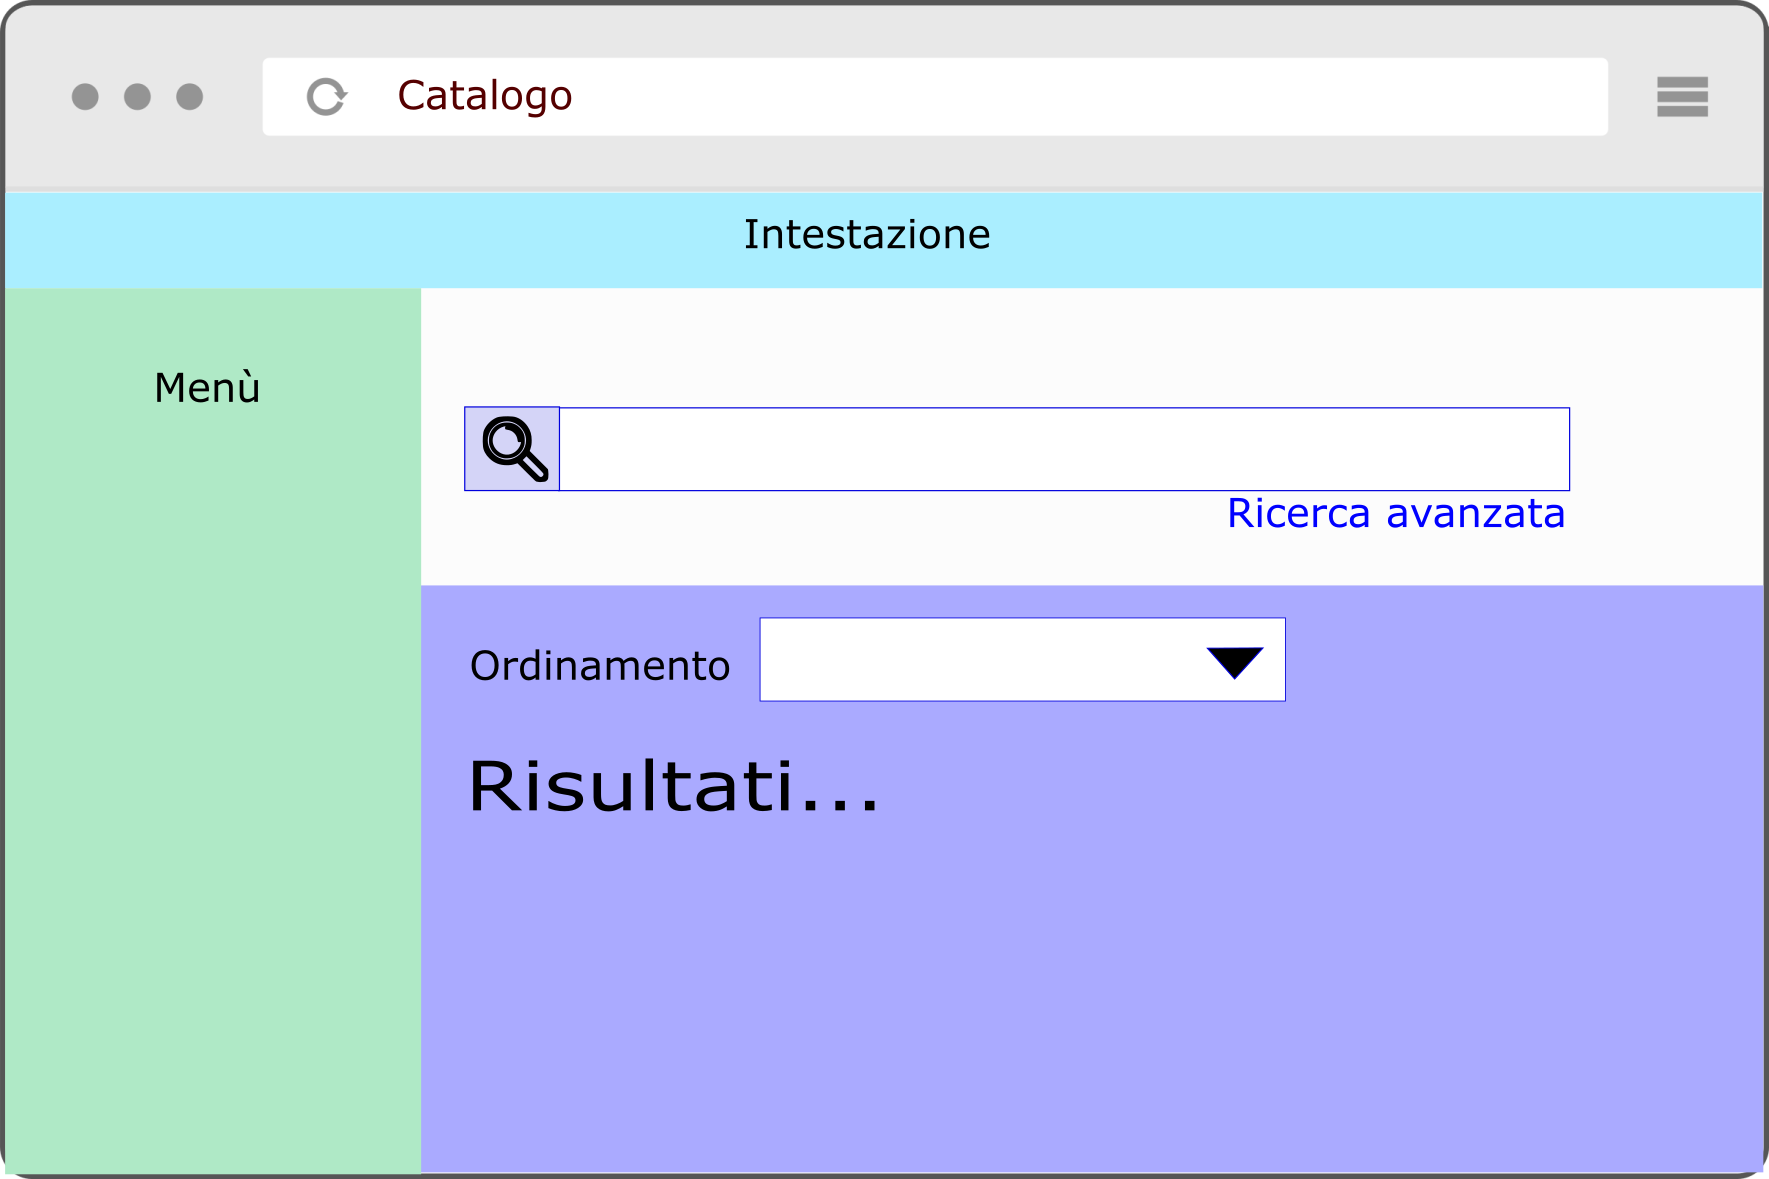
\includegraphics[width= 14cm]{immagini/catalogo.png}
	\caption{Catalogo dei libri}
\end{figure}

\subsection{Dettaglio}
\textbf{[descrizione dettagli]}
\begin{figure}[H]
	\centering
	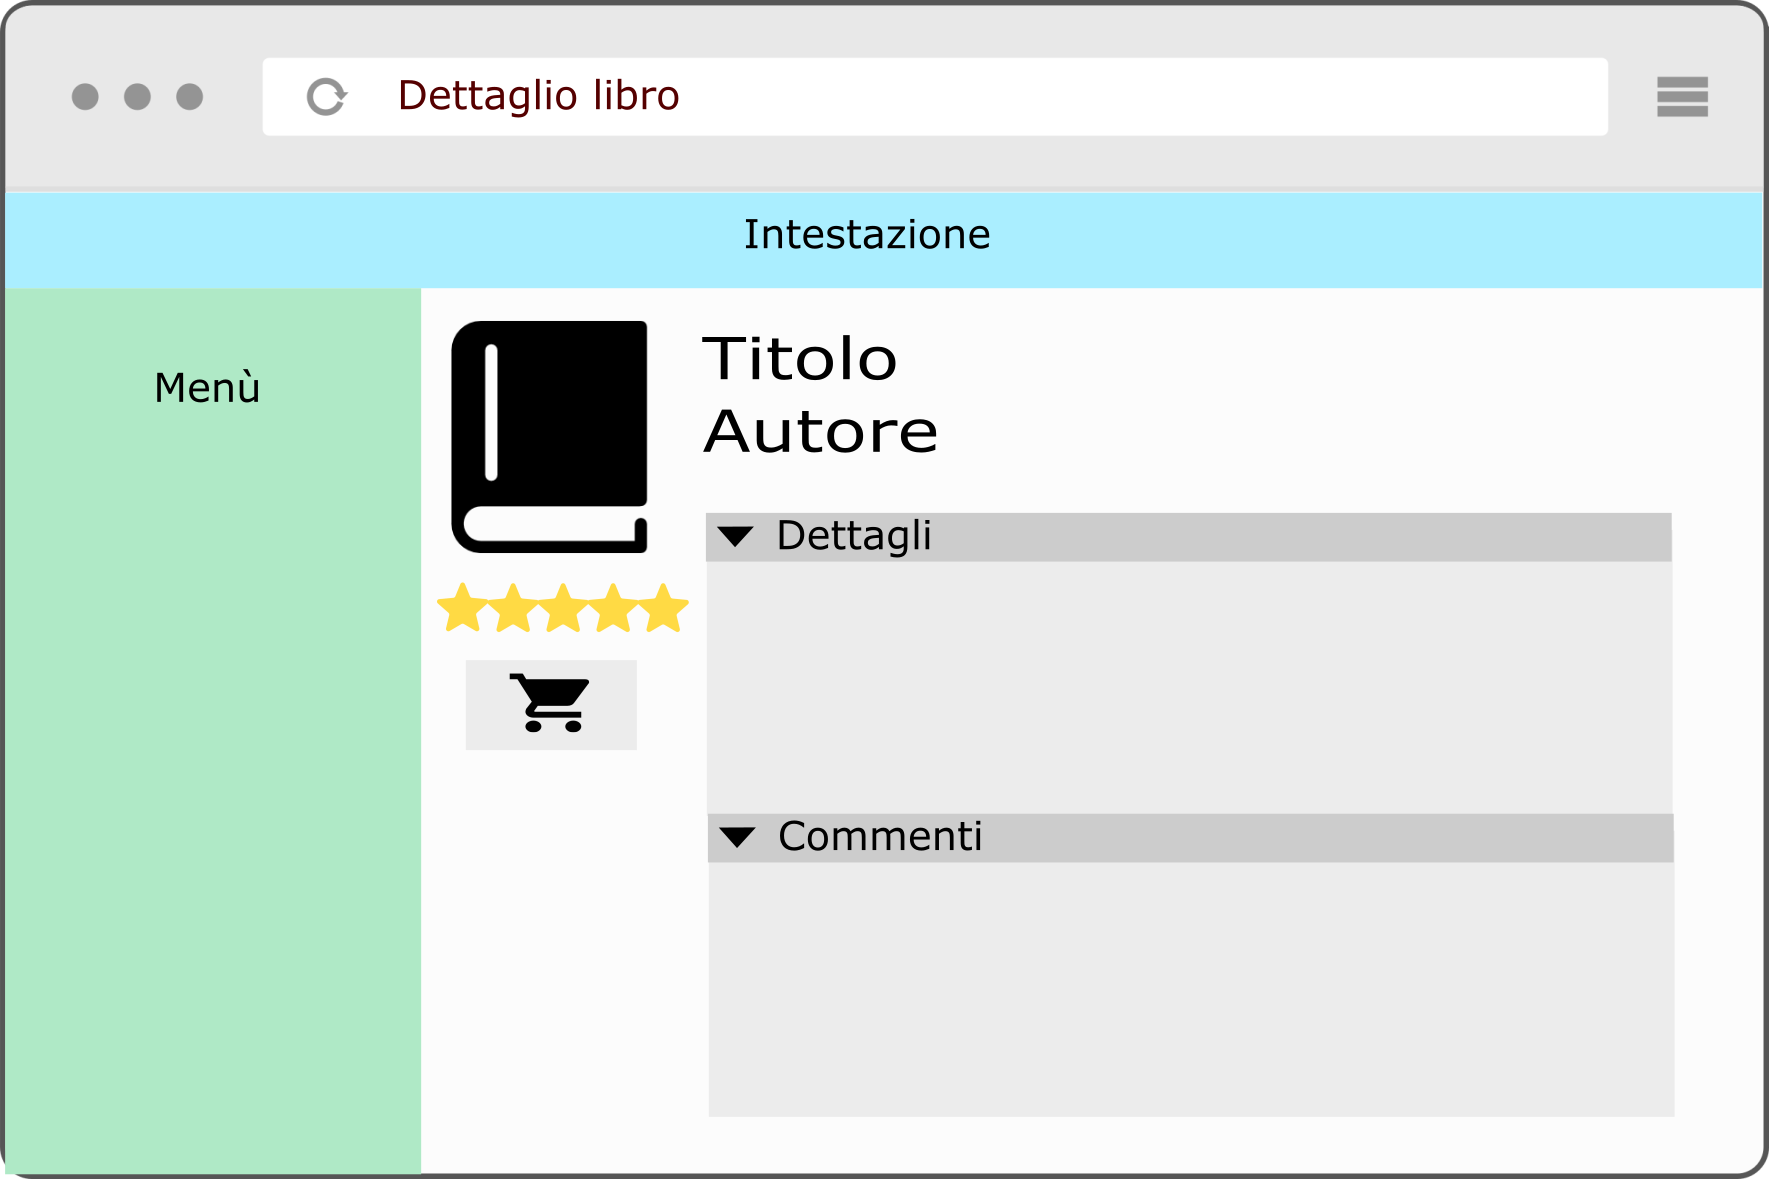
\includegraphics[width= 14cm]{immagini/dettaglio.png}
	\caption{Visione di dettaglio dei libri}
\end{figure}

\subsection{Servizi}
[descrizione servizi..]
\begin{figure}[H]
	\centering
	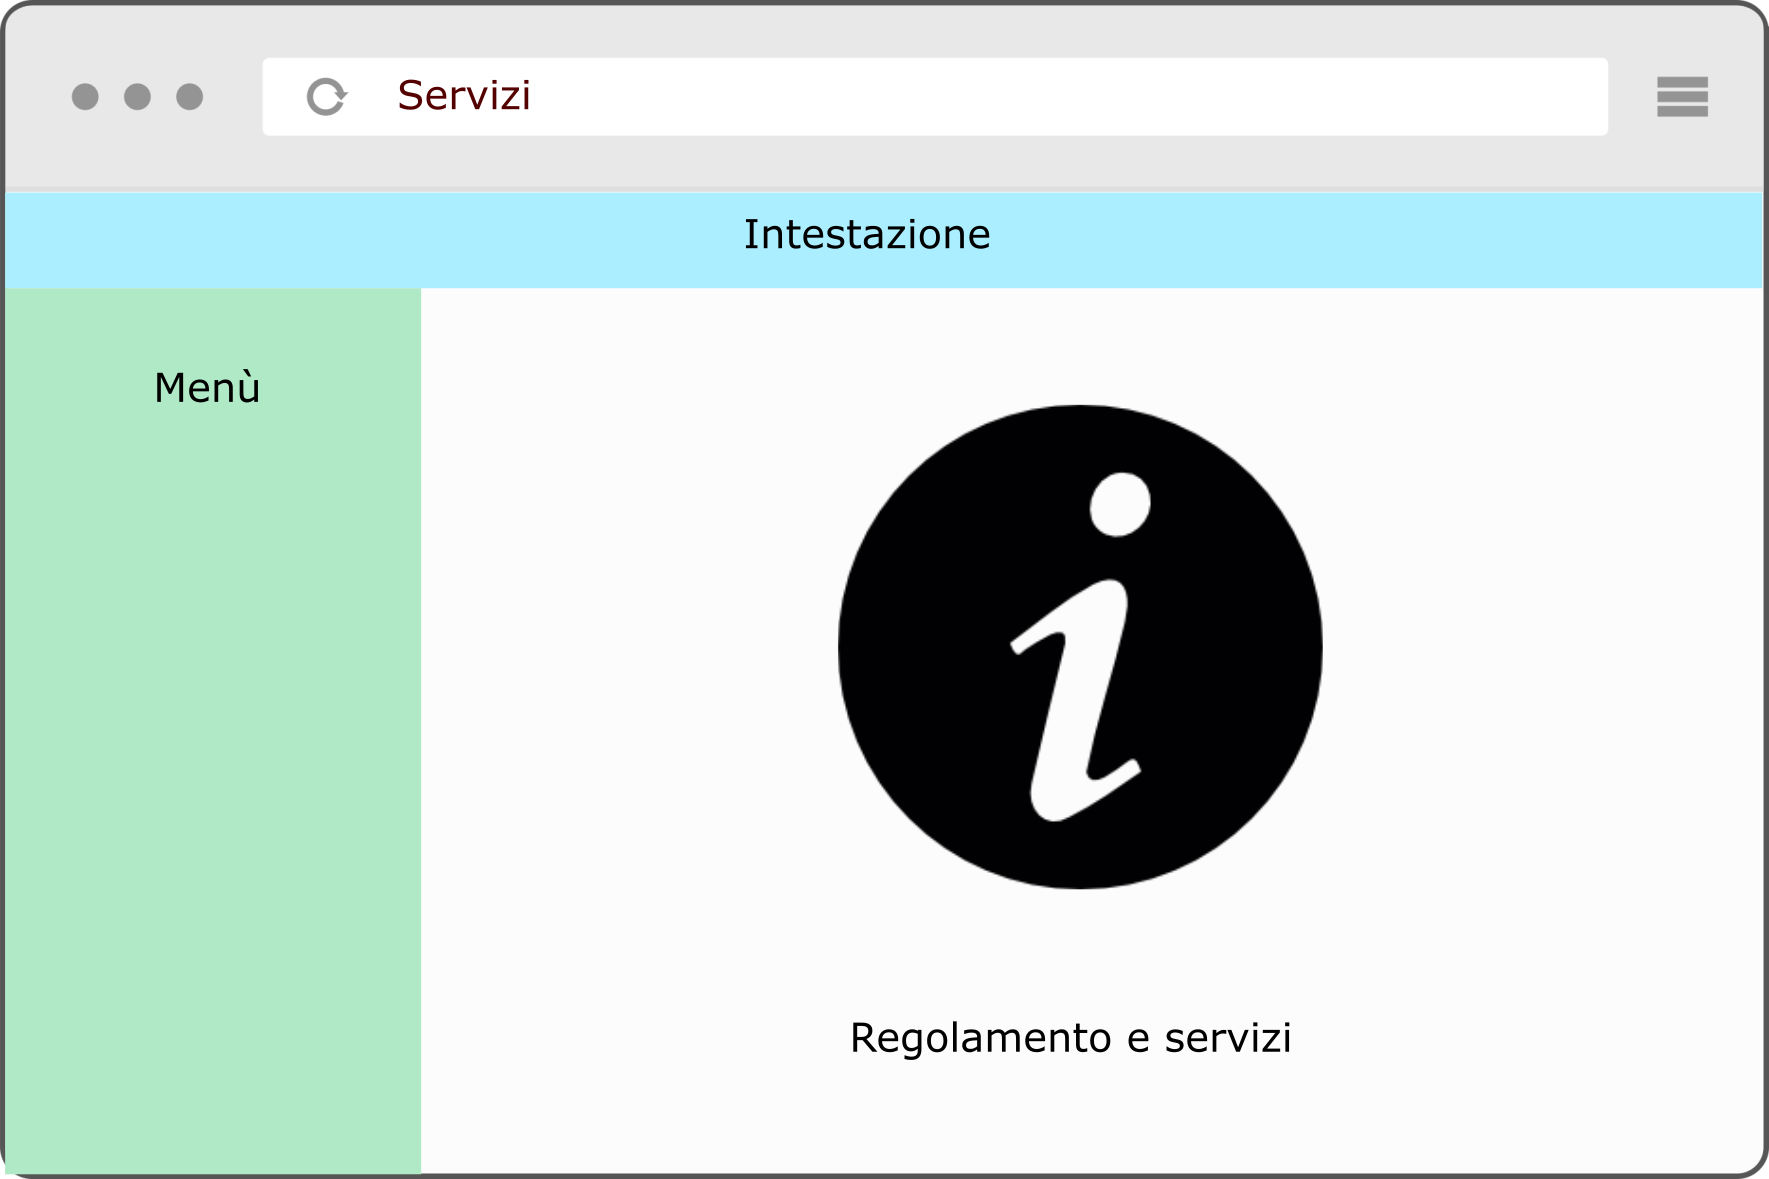
\includegraphics[width= 14cm]{immagini/servizi.png}
	\caption{Servizi offerti e regolamento}
\end{figure}

\subsection{Contatti}
[descrizione contatti..]
\begin{figure}[H]
	\centering
	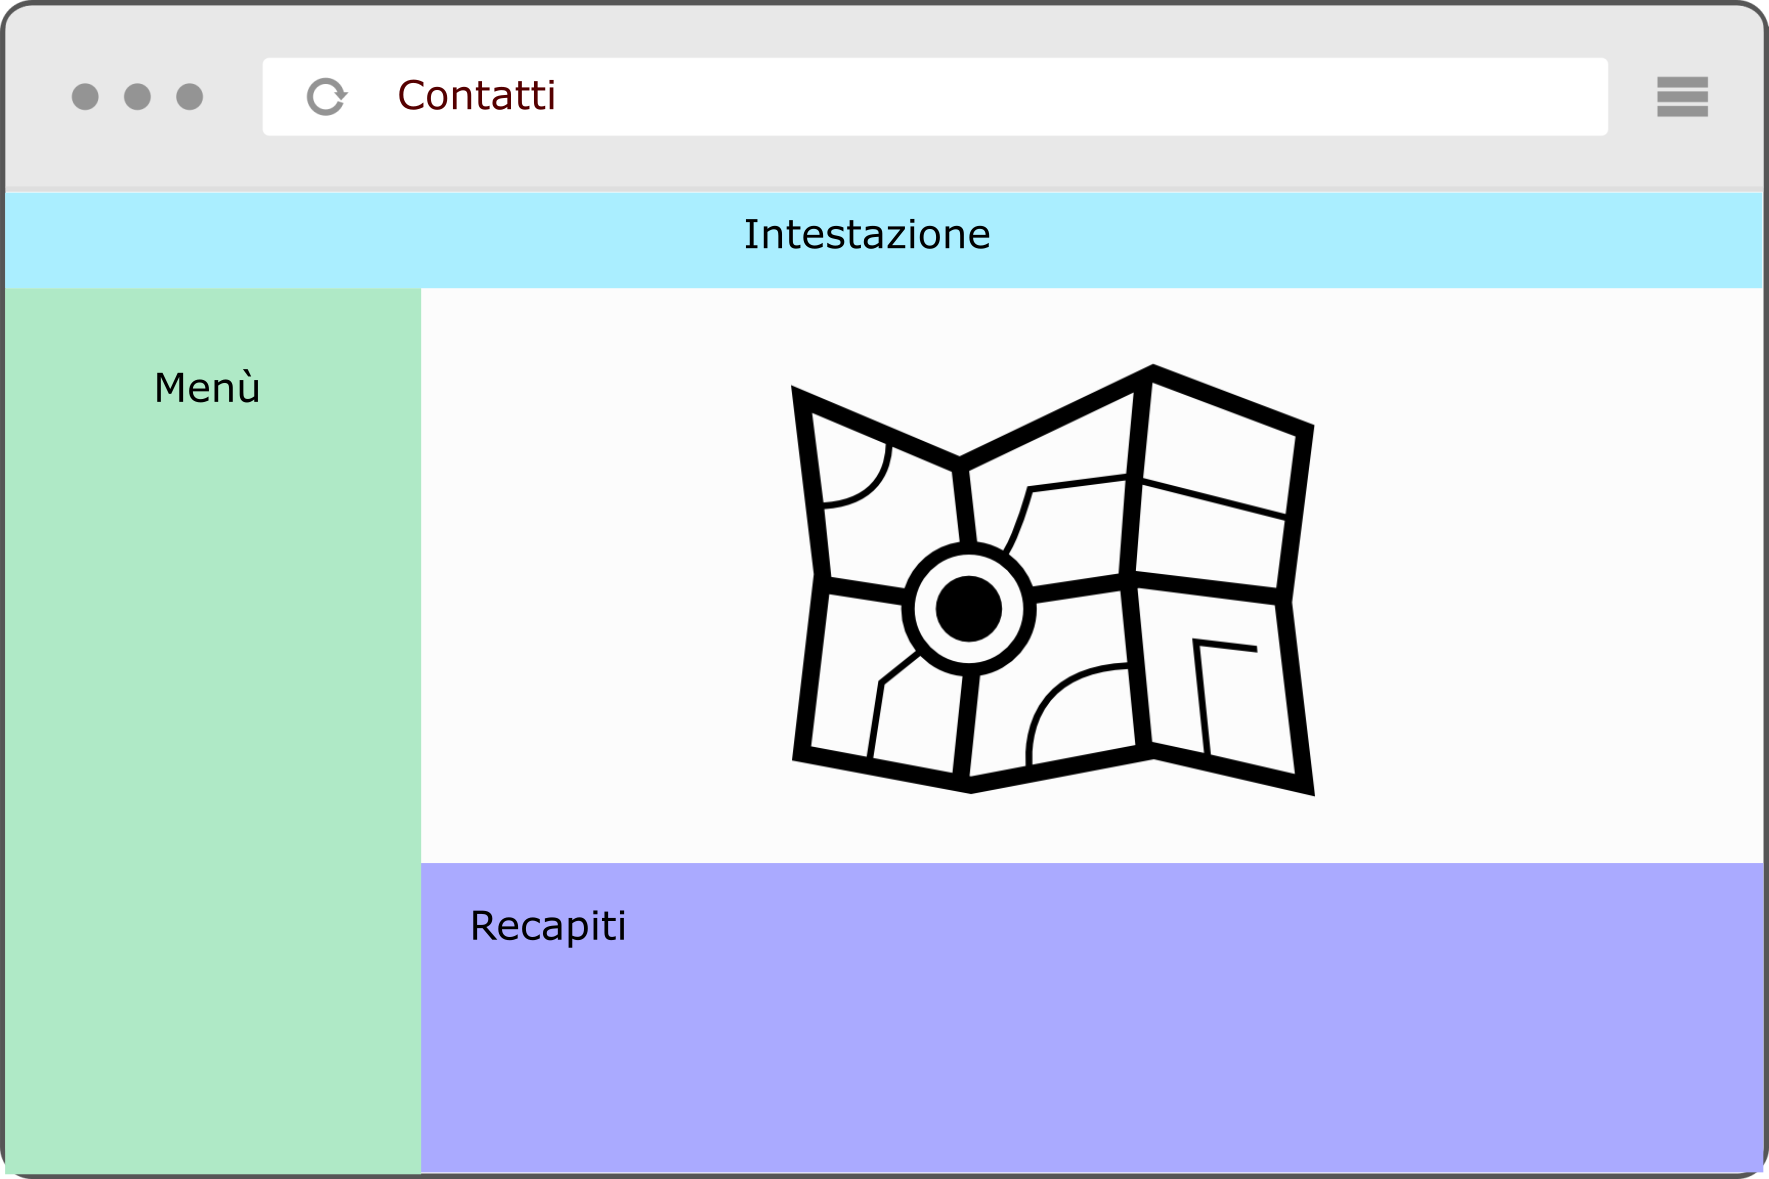
\includegraphics[width= 14cm]{immagini/contatti.png}
	\caption{Indicazioni e recapiti}
\end{figure}

\subsection{Prenotazione}
[descrizione prenotazione..]

\subsection{Gestione prestiti}
[descrizione gestione prestiti..]

\subsection{Profilo utente}
[descrizione profilo utente..]

\subsection{Amministrazione}
\subsubsection{Conferma account}
[descrizione conferma account..]

\subsubsection{Inserimento libro}
[descrizione inserimento libro..]

\subsubsection{Rimozione commento}
[descrizione rimozione commento..]

